\section{Phương pháp đề xuất}
\subsection{Kiến trúc dữ liệu lớn}
\subsection{Ứng dụng web}
\subsubsection{Công nghệ được sử dụng }
\subsubsection{Flask}

Flask là một framework phát triển web nhẹ, đơn giản và dễ sử dụng trong Python.
Được tạo ra bởi Armin Ronacher, Flask thuộc dạng "micro-framework", nghĩa là nó
không đi kèm với quá nhiều tính năng mặc định, cho phép lập trình viên tự do lựa
chọn và tích hợp các thành phần mà họ cần. Đặc điểm chính của Flask:
\begin{itemize}
    \item Nhẹ nhàng và dễ mở rộng: Flask chỉ cung cấp những tính năng cơ bản như
        định tuyến URL, quản lý yêu cầu và phản hồi HTTP. Các tính năng nâng cao như cơ sở dữ liệu, xác thực hay quản lý phiên người dùng có thể được thêm qua các thư viện mở rộng.
    \item Dễ học và sử dụng: Flask được thiết kế với cú pháp đơn giản, dễ đọc,
        phù hợp cho cả người mới học lập trình web và các chuyên gia phát triển.
    \item Không gò bó: Không giống như các framework lớn như Django, Flask không
        ép buộc bạn phải tuân theo một kiến trúc cụ thể. Bạn có thể tự do tổ chức dự án theo cách riêng của mình.
\end{itemize}

\subsubsection{PostgreSQL}

PostgreSQL (thường được gọi là Postgres) là một hệ quản trị cơ sở dữ liệu quan
hệ mã nguồn mở mạnh mẽ và linh hoạt. Được phát triển từ năm 1986 tại Đại học
California, Berkeley, Postgres đã trở thành một trong những hệ thống cơ sở dữ
liệu phổ biến và được tin cậy nhất hiện nay. Đặc điểm nổi bật của PostgreSQL:
\begin{itemize}
    \item Hệ quản trị cơ sở dữ liệu quan hệ đối tượng (ORDBMS): PostgreSQL hỗ
        trợ không chỉ dữ liệu quan hệ truyền thống mà còn có khả năng lưu trữ và xử lý dữ liệu dạng đối tượng, JSON, XML, và các loại dữ liệu không gian (spatial data).

    \item Mã nguồn mở và miễn phí: PostgreSQL là một dự án mã nguồn mở, nghĩa
        là bạn có thể sử dụng, chỉnh sửa và phân phối mà không mất phí. Nhiều công ty lớn sử dụng Postgres làm nền tảng cơ sở dữ liệu của họ.

    \item Hiệu suất cao: PostgreSQL được tối ưu hóa để xử lý khối lượng lớn dữ
        liệu và thực hiện các truy vấn phức tạp một cách hiệu quả.

    \item Hỗ trợ đa nền tảng: PostgreSQL có thể chạy trên nhiều hệ điều hành
        như Linux, Windows, macOS, và các hệ thống UNIX khác.

    \item Cộng đồng lớn: PostgreSQL có một cộng đồng phát triển và người dùng
        đông đảo, cung cấp tài liệu, hỗ trợ kỹ thuật và nhiều tiện ích mở rộng.
\end{itemize}

\subsubsection{Thiết kế cơ sở dữ liệu}

Dữ liệu của MOOCCubeX được lưu trữ dưới các file json và txt, vì vậy nhóm cần
phải chuyển các file này vào cơ sở dữ liệu của PostgreSQL. Trước hết, nhóm cần phải
thiết kế một lược đồ cơ sở dữ liệu để lưu trữ các thông tin cần thiết cho việc demo:

\begin{figure}[h]
    \centering
    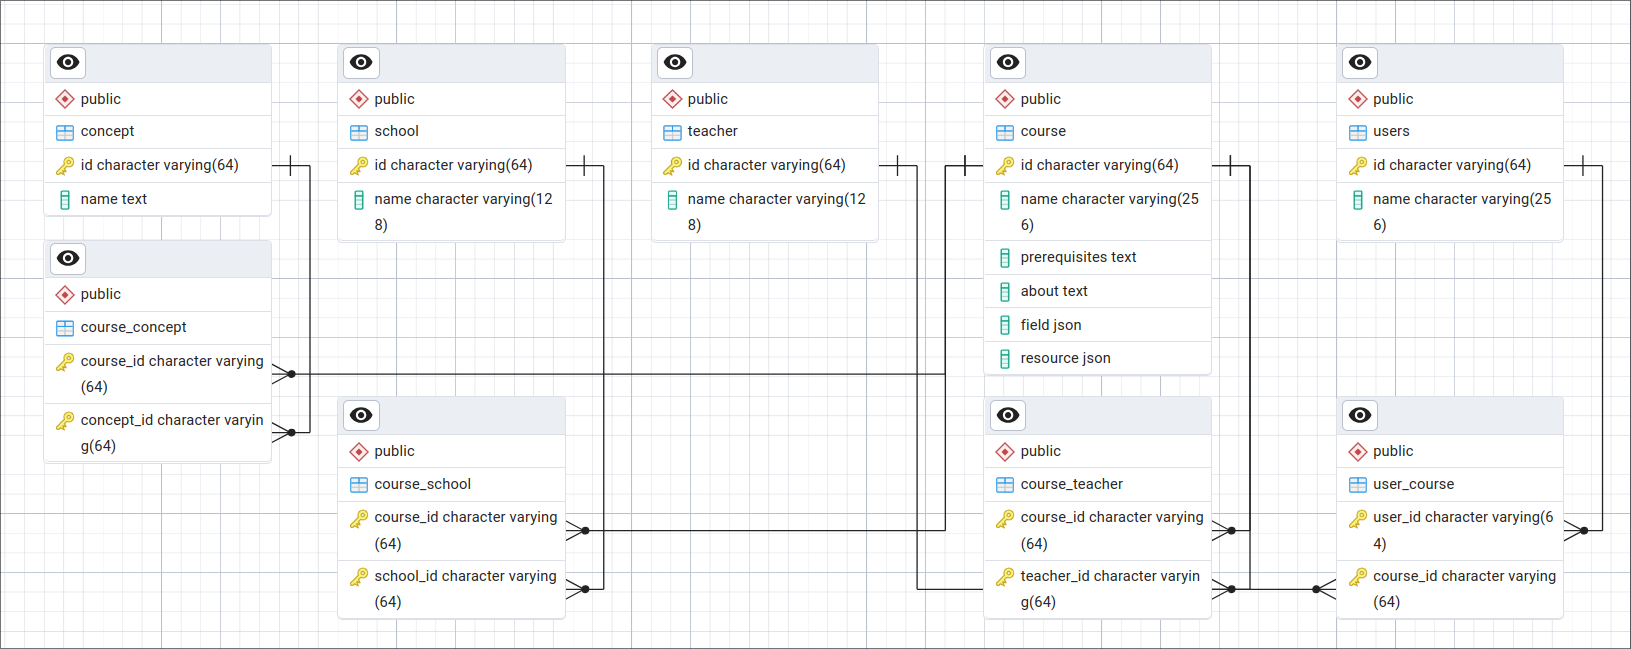
\includegraphics[width=0.8\textwidth]{figures/72.png}
    \caption{Cơ sở dữ liệu}
\end{figure}

\subsubsection{Thiết kế giao diện}
